%************************************************
\chapter{Einführung}\label{ch:introduction} %************************************************
%*****************************************
%*****************************************
%*****************************************
%*****************************************
%*****************************************
\section{Einleitung}\label{sec:einleitung}
Notes:

\begin{itemize}
    \item solarwinds as introduction
    \item use advances of sequence detection from NLP
    \item NIDS vs. HIDS
    \item signature vs.\ anomaly based
    \item Forrest et al 1996 erstmals syscall traces
    \item low level interactions between program and kernel
    \item syscall traces dont stop execution contrary to debuggers
    \item tracing virtually every linux without modifying source code
    \item whole system behaviour visible in kernel
\end{itemize}

Angriffe auf Computersysteme werden frequenter.
Die häufig verwendeten auf Signaturen basierenden Abwehrmechanismen reichen nicht aus um viele drohende Gefahren abzuwenden.
Dies liegt hauptsächlich daran, dass weder Abwandlungen von bekannten Angriffen, noch unbekannte Angriffe erkannt werden können.
Zusätzlich müssen die Signaturen für jeden Angriffsvektor einzeln eingefügt werden\marginpar{vgl. \autoref{sec:Datenanalyse}}.
Ein wesentlicher Vorteil liefert hier die Angriffserkennung über Anomalien.
Im Gegensatz zu dem erwähnten signaturbasierten Ansatz, muss nicht jeder Angriff der abgewehrt werden soll bekannt sein.
%Stattdessen wird versucht das Normalverhalten eines Systems zu ermitteln und jegliche Abweichung als Anomalie und damit als Angriff einzustufen.
Stattdessen wird versucht ein Modell des zu erwartenden Normalverhalten des Systems zu erstellen.
Mit dem erstellten Modell sollen dann, möglichst in Echtzeit, Abweichungen bzw. Anomalien des erwarteten Verhalten signalisiert werden.

Die Bedeutsamkeit der Erkennung von bisher unbekannten Angriffe wird ebenfalls durch das \ac{BSI} bestätigt.
Das \ac{BSI} berichtet, dass im Berichtzeitraum\marginpar{Juni 2020 bis Mai 2021} die Schadprogramm-Varianten um rund 144 Millionen zugenommen haben\marginpar{vgl.\autoref{ch:zero-day}}, was einer Steigerung von 22\% gegenüber dem Zeitraum des vorigen Berichts bedeutet.~\cite{BSI}.

\begin{chart}

    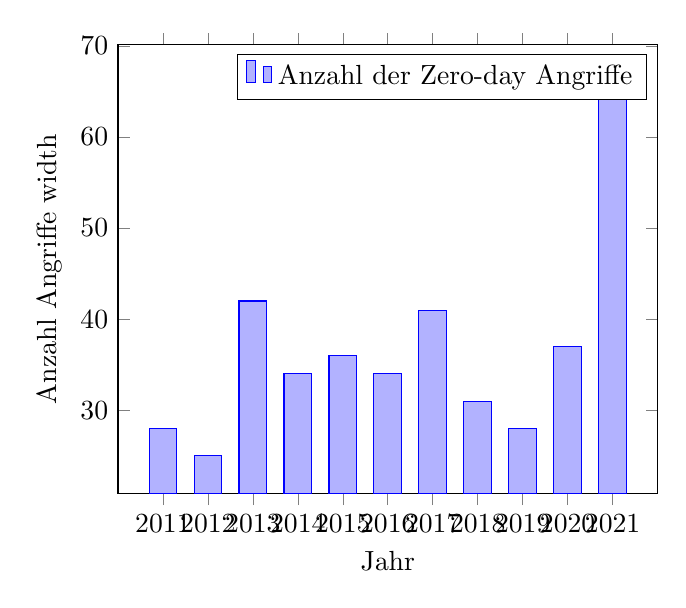
\begin{tikzpicture}
     
        \begin{axis} [ybar,
            /pgf/number format/1000 sep={},
            xmin=2010,
            xmax=2022,
            xtick=data,
            xlabel={Jahr},
            ylabel={Anzahl Angriffe}
            width=16cm,
            legend cell align={left}]
        \addplot coordinates{
            (2011,28) 
            (2012,25) 
            (2013,42) 
            (2014,34) 
            (2015,36) 
            (2016,34) 
            (2017,41) 
            (2018,31) 
            (2019,28) 
            (2020,37) 
            (2021,66) 
        };

        \legend{Anzahl der Zero-day Angriffe}
    \end{axis}
     
    \end{tikzpicture}
  \caption{A chart test}\label{ch:zero-day}
\end{chart}

% Laut eines Berichts von Symantec aus dem Jahr 2013 werden die von den Angriffen ausgenuetzten Sicherheitsluecken im Schnitt erst nach 312 Tagen geschlossen.

Speziell werden in dieser Arbeit \ac{HIDS} verwendet, das sie gegenueber den \ac{NIDS} feingranularer sind und auch interne Attacken erkennen koennen.
Nun bieten verschiedene Systeme unterschiedliche Möglichkeiten das ihnen zugrunde liegende Verhalten zu beschreiben. 
Eine häufig verwendete Information für die Charakterisierung bieten zum Beispiel System-Logs~\cite{HE}.

In dieser Arbeit werden System-Calls verwendet.
Sie bieten eine sehr abstrakte Betrachtung auf Betriebssystemebene.
Programme auf einer Festplatte können meist erst Schaden anrichten, sobald sie ausgeführt werden.
Dabei führen sie betriebssystemspezifische System-Calls aus, welche über verschiedene Tools wie zum Beispiel Sysdig~\cite{SYSDIG} ausgelesen werden können.
Die Schwierigkeit im Vergleich zu dem Untersuchen der Logs besteht darin, die großen Datenmengen zu bewältigen, welche schon bei kleineren Anwendungen anfallen.
Die Probleme in der Verarbeitung von sehr großen Datenmengen konnten unter anderem durch die Verwendung selbst lernender Algorithmen erfolgreich angegangen werden.
Im realen Einsatz solcher Verteidigungsmechanismen besteht eine weitere Schwierigkeit darin, dass das \ac{IDS} Zugriff auf den Kernel des zu überwachenden Systems benötigt.
Diese wird in dieser Arbeit allerdings nicht behandelt, da lediglich die Algorithmen selbst, jedoch nicht die praktische Umsetzung in einem potentiellen Betrieb betrachtet wird.

In verschiedenen Arbeiten wurden bereits die Abfolge von System-Calls betrachtet, doch nur in wenigen Arbeiten werden auch die Parameter zur Anomalieerkennung verwendet. Eine der ersten Arbeiten von Forrest et al.~\cite{FORREST} betrachtet lediglich die Sequenzen der System-Calls.
Maggi et al.\ verwenden zusätzlich auch Parameter und verweisen in ihrer Arbeit~\cite{MAGGI} auf diverse verschiedene Ansätze.
In dieser Arbeit soll versucht werden die Hinzunahme eines Parameters, wie zum Beispiel den Dateipfad (sofern vorhanden) bei schreibenden und lesenden Befehlen, mit Hinblick auf die Erkennungsquote des \ac{IDS} zu untersuchen.

Nachdem definiert wurde welche Information untersucht wird, stellt sich zu Beginn der Entwicklung einer Anomalieerkennung die Frage, wie das Normalverhalten der Systeme erfasst werden soll.
Abstrakt betrachtet werden bei der Untersuchung von System-Calls zeitvariante und potentiell multivariate Datenstreams betrachtet, sofern neben der eigentlichen Sequenz noch weitere Parameter betrachtet werden.
Besonders erfolgreich haben sich dabei Long-Short-Term-Memory (LSTM) Netzwerke gezeigt.
Sie haben den Vorteil auch Zusammenhänge mit größerer zeitlicher Verzögerung noch zu erkennen~\cite{HOCHREITER} und können in unterschiedlichsten Architekturen einen Nutzen bringen. %\cite{SMAGULOVA}.

\section{Zielsetzung}

In dieser Arbeit sollen zwei Forschungsfragen verfolgt werden.
\begin{itemize}
    \item Kann der Erfolg von LSTM-Netzwerken in verschiedenen Bereichen auf die Erkennung von Anomalien in der Cyber-Sicherheit übertragen werden?
    \item Kann die Zunahme von Parametern bei der Anomalieerkennung mittels System-Calls eine Verbesserung bringen?

        $\rightarrow$ Welche Parameter kommen in Frage?
\end{itemize}
%Des Weiteren wird, je nach Erfolg der ersteren Fragen noch optional folgendes untersucht:
%\begin{itemize}
%    \item Können aktuelle Verbesserungen des Lernverhaltens durch GAN auch hier Anwendung finden?
%    \begin{itemize}
%        \item MAD-GAN \cite{LI}
%        \item VAE-MAD-GAN \cite{NIU}
%    \end{itemize}
%\end{itemize}

Um diese Forschungsfragen angemessen behandeln zu können müssen zunächst Grundlagen aus verschiedenen Bereichen gelegt werden.
Zum einen werden unterschiedliche Herangehensweisen zur Überwachung von Systemen betrachtet und erläutert wieso es für diese Anwendung sinnvoll ist eine Host-Based Intrusion Detection zu wählen.
Speziell soll auch beschrieben werden, warum sich System-Calls zur Überwachung von Computersystemen eignen.
Des Weiteren müssen Grundlagen für die in dem verwendeten Algorithmus verwendeten Techniken gelegt werden.
Dazu gehören Hauptsächlich Grundlagen zu rekurrenten neuronalen Netzen (RNN) sowie die Erweiterungen der LSTM Netzwerke.

Ein großer Teil der Implementierungsarbeit jedoch wird die Vorverarbeitung der Daten darstellen.
Diese soll mit der genaueren Untersuchung der Zusammensetzung der Techniken für den Algorithmus in einem weiteren Kapitel dargestellt werden.
Nachdem die verwendete Software analysiert wurde, wird eine Auswertung auf dem LID-DS~\cite{LID-DS} Datensatz durchgeführt.
Dieser bietet den Vorteil, dass in einer reproduzierbaren Art System Calls aufgenommen wurden.
Des Weiteren werden zusätzlich die System Call Parameter, wie zum Beispiel die \textit{Thread ID} zur Verfügung gestellt.

Im letzten Teil der Arbeit soll dann eine Schlussfolgerung aus den zuvor gewonnenen Ergebnissen gezogen werden. 
Hauptsächlich sollen die gestellten Forschungsfragen untersucht werden.
Konnte mit einem hinzugezogenen Parameter ein Mehrwert erzielt werden?
Bieten sich LSTM-Netzwerke auch für die Anomalieerkennung im IT-Sicherheitsbereich an?
